\section{Durchführung}
\label{sec:Durchführung}

Der grundlegende Aufbau des Versuches ist in Abbildung \ref{fig:aufbau} zu sehen. Die Bauteile sind auf einer optischen Schiene beweglich.

\begin{figure}
  \centering
  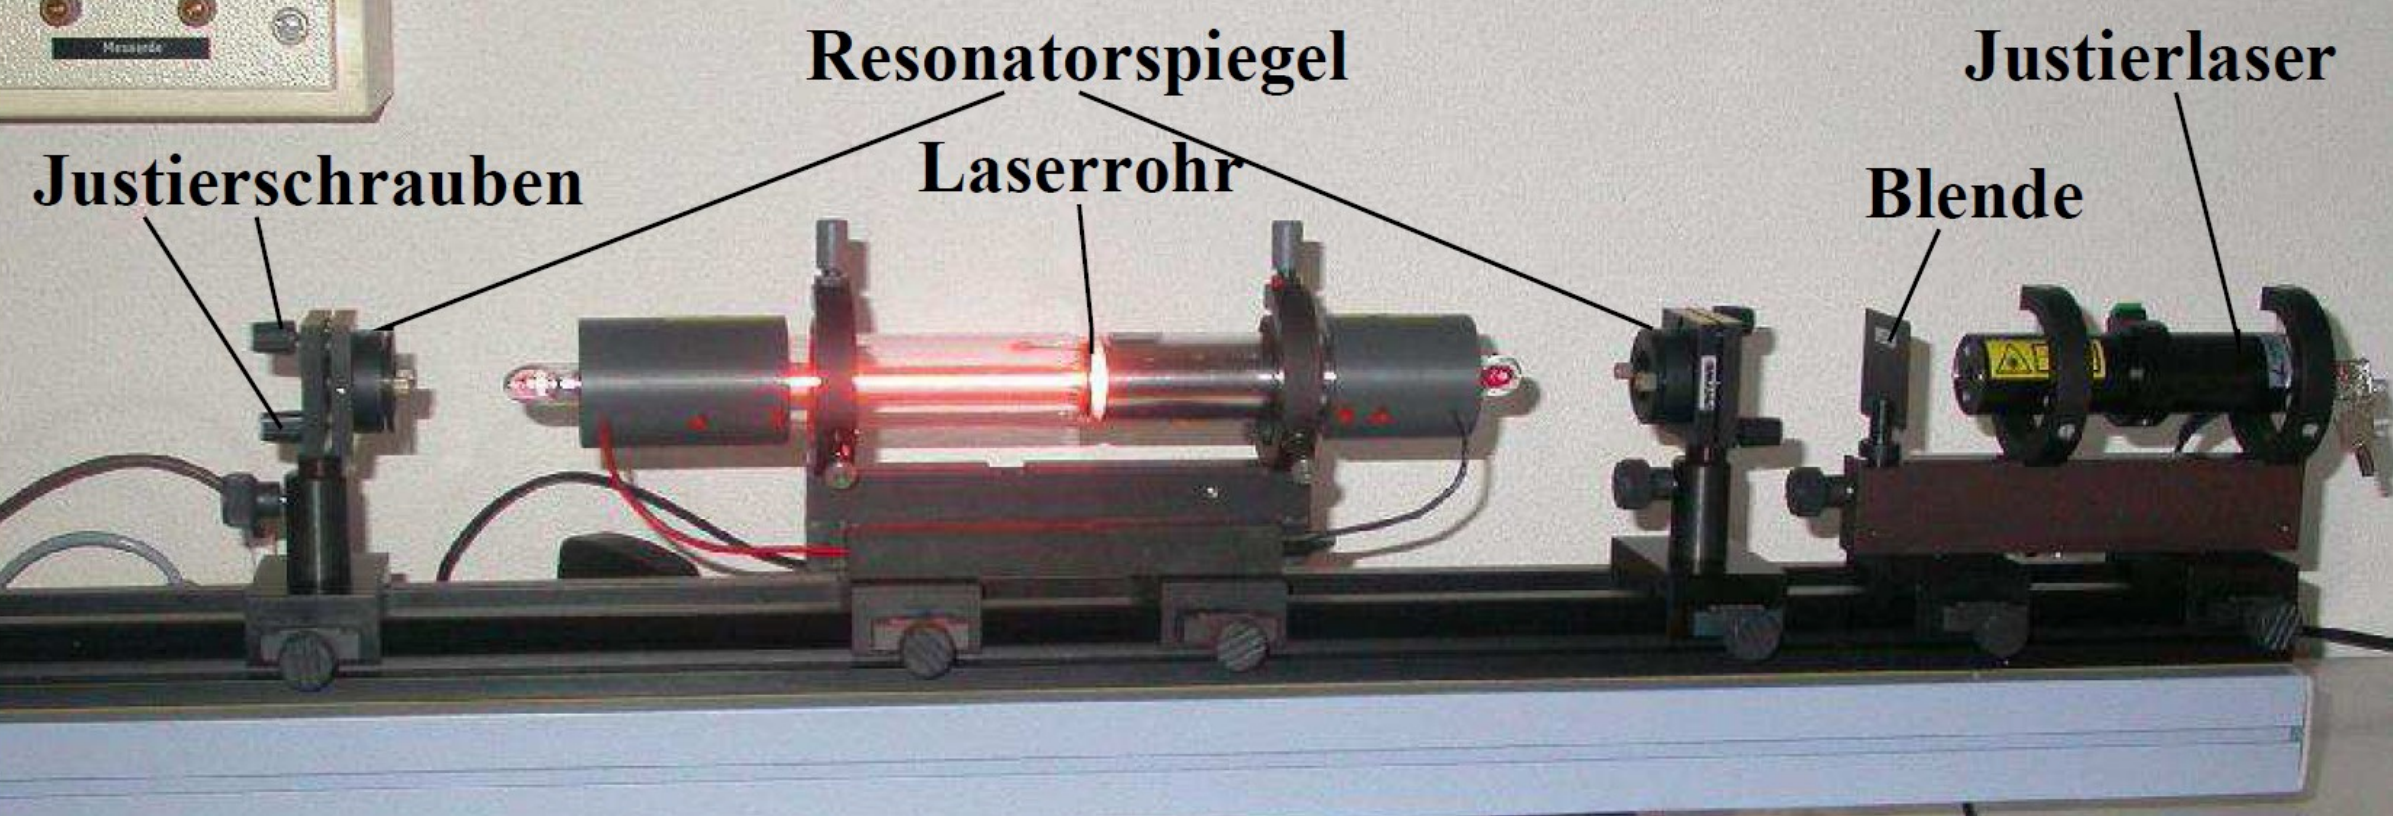
\includegraphics[width=\textwidth]{data/aufbau.png}
  \caption{Foto der Apparatur mit ihren wesentlichen Komponenten \cite{Anleitung_neu}.}
  \label{fig:aufbau}
\end{figure}

Eine genaue Justierung des Lasers ist nötig, um einen stabilen Laserstrahl zu erhalten. Der Justierlaser kann für diesen Zweck verwendet werden. Die Justierschrauben der Spiegel werden so eingestellt, dass der reflektierte Laserstrahl mittig auf die Blende zurückfällt. Ein erneutes Justieren der Schrauben ist nötig, nachdem die Spiegel auf den gleichen Abstand zum Laserrohr eingestellt wurden. Während den eigentlichen Messungen ist der Justierlaser außer Betrieb.

Die Durchführung dieses Versuches ist in vier Teile gegliedet, die im Nachfolgenden beschrieben werden.

Zunächst ist die Stabilitätsbedingung zu überprüfen. Dazu werden zwei Messreihen der Lichtintensität an einer Photodiode, ausgedrückt durch eine angezeigte Stromstärke, in Abhängigkeit der Länge des Laseraufbaus, also des Resonatorspiegelabstandes, aufgenommen. Bei der einen Messreihe wurde ein konkav-flaches Spiegelpaar verwendet, bei der anderen ein Paar aus konkaven Spiegeln. Die beiden konkaven Spiegel haben eine Brennweite von $\SI{1400}{\milli\meter}$. Eine häufige Nachjustage ist nötig, um zu gewährleisten, dass stets möglichst ein Maximum der Intensität für die gegebene Apparaturlänge aufgezeichnet wird.

Danach werden die verschieden transversalen Moden des Lasers untersucht. Um die Moden quantitativ zu messen, wird der Strahl durch eine Streulinse, die auf der optischen Schiene in den Strahlengang gestellt wird, aufgefächert. Durch Verschieben der Photodiode, die mit einer Skala versehen ist, kann dann die Intensität entlang einer $x$-Achse vermessen werden. \\
Da die TEM$_{\mathrm{0,0}}$ Mode das Modenspektrum dominiert, wird ohne weiteres Zubehör die Intensität gemessen. Danach wird die Messung wiederholt, nachdem ein feiner Draht in den Strahlengang gestellt wurde. Dieser dient dazu, höhere Moden, die sonst stark unterdrückt sind, sichtbar zu machen. Liegt der Draht in einem Knotenpunkt einer bestimmten Mode, so kann nur diese Mode frei schwingen. Es wird die TEM$_{\mathrm{0,1}}$ Mode sichtbar gemacht.

Im dritten Teil des Versuchs wird die Polarisation des Laserstrahls untersucht. Dazu wird ein Polarisationsfilter, dessen Einstellung sich zwischen 0 und 360$\,°$ variieren lässt, in den Strahlengang gestellt und eine Messreihe der Intensität in Abhängigkeit des eingestellten Winkels aufgenommen.

Zuletzt soll noch die Wellenlänge des Lasers bestimmt werden. Zu diesem Zweck wird die Beugung des Strahls an einem Gitter betrachtet, das vor einem Schirm auf die optische Schiene gestellt wird. Durch Einstellen eines großen Abstands zwischen Gitter und Schirm wird erreicht, dass nur das nullte und die beiden ersten Beugungsmaxima auf dem Schirm zu sehen sind, um eine hohe Genauigkeit zu erreichen. Der Abstand der beiden ersten Maxima vom nullten Maximum werden aufgezeichnet.
